\documentclass[9pt,a4paper,twocolumn]{article}
\usepackage[margin=0.7in]{geometry}
\usepackage{hyperref}
\usepackage[final]{pdfpages}
\usepackage{subcaption}
\usepackage{cite}

\title{An Analysis of the Portuguese Section of Wikipedia}

\author{Daniel Ramos \\ 81620 \and Miguel Tavares \\ 83528 \and Ricardo Brancas  \\ 83557}

\begin{document}
\maketitle

\section{Introduction}
The goal of this project is to analyse and characterize a real world network, and to  get 
acquainted with tools and methods which will be useful in following endeavours.
As such, we have chosen to analyse a snapshot of the Portuguese section of Wikipedia \cite{dataset};
we have chosen such a large network in order to get familiarized with tools such as Webgraph \cite{webgraph}.

To analyse our data we use Webgraph, including snippets of code made available
by Prof. Alexandre Francisco \cite{aplf}.

%TODO

\section{Methods}
The network was originally represented as an edge list which was subsequently converted in an adjacency list (ASCII Graph), by use of a simple \texttt{C++} program, as this is the input
format for Webgraph's compression algorithms. 





\section{Results}

Our network contains $1\,603\,222$ vertices and $49\,021\,409$ edges. Both the minimum in and out degrees are $0$, the maximum in degree is $207254$ while the maximum out degree is $12237$, finally the combined average degree of approximately $61.15$.
\vspace{1\baselineskip}

In figure ~\ref{fig:inddist}/~\ref{fig:outddist} we present the cumulative in/out degree distribution and its approximate power law regression. The regression was obtained using a simplified method based on the one described by Clauset et al. \cite{Clauset2009}.

Figure \ref{fig:sccdist} shows the number of strongly connected components with respect to their cardinality. We notice a giant strongly connected component, as would be expected.

Figure \ref{fig:neighfun} 


\begin{figure}[h]
	\centering
	\begin{subfigure}{.45\textwidth}
		\centering
		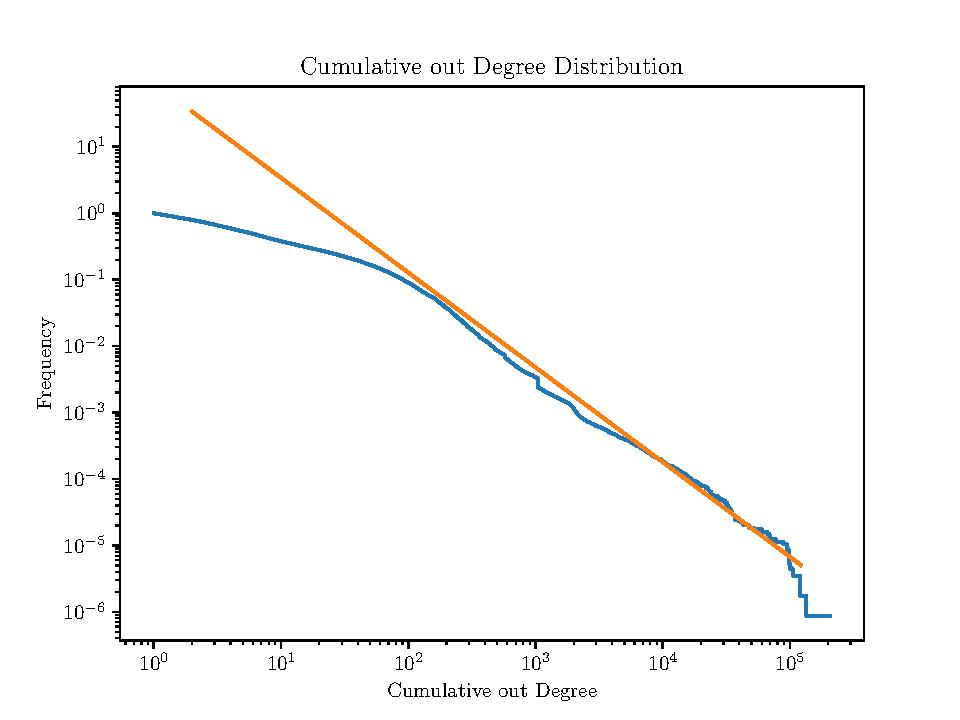
\includegraphics[width=\linewidth]{wikipedia_pt_in.pdf}
		\caption{Cumulative in-degree distribution.}
		\label{fig:inddist}
	\end{subfigure}
	\begin{subfigure}{.45\textwidth}
		\centering
		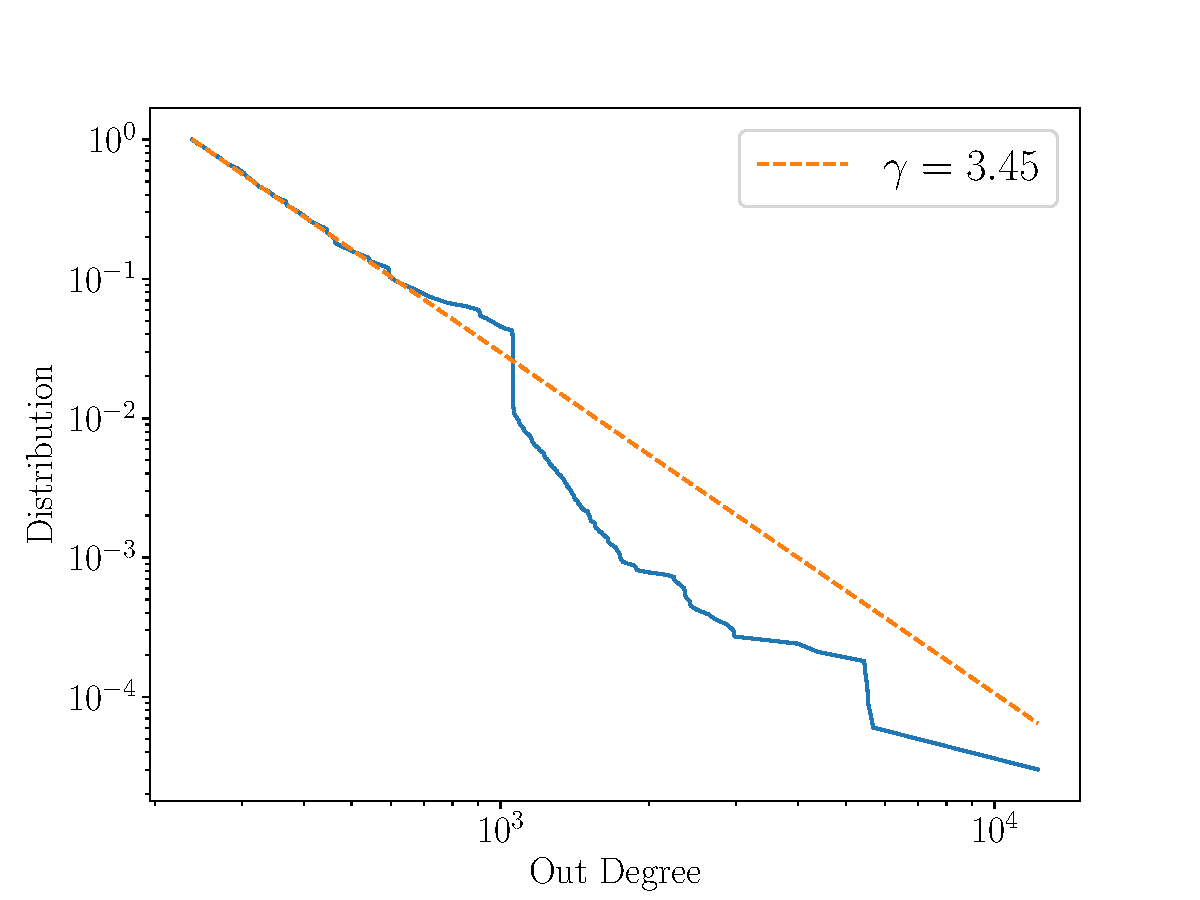
\includegraphics[width=\linewidth]{wikipedia_pt_out.pdf}
		\caption{Cumulative out-degree distribution.}
		\label{fig:outddist}
	\end{subfigure}
	\caption{Degree distributions.}
\end{figure}

\begin{figure}[h]
	\centering
	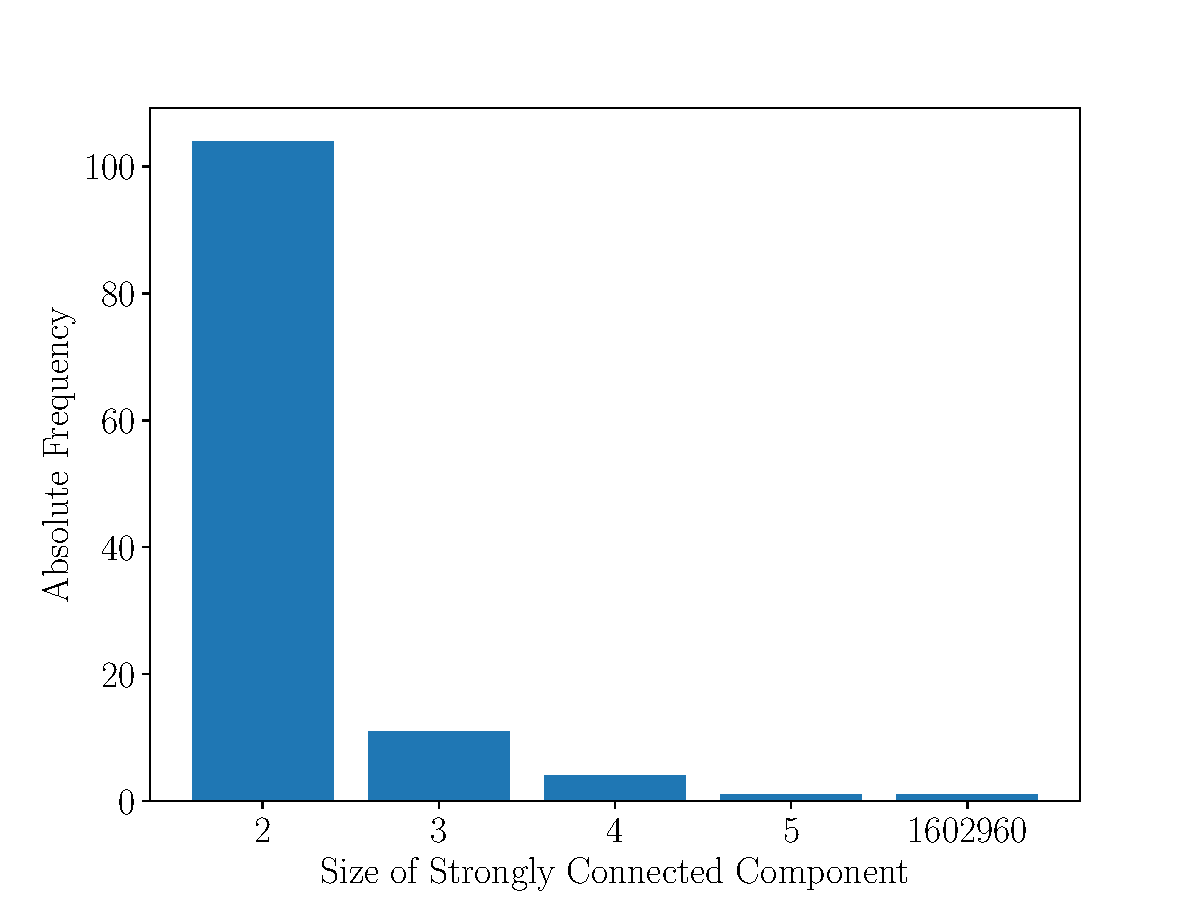
\includegraphics[width=\linewidth]{wikipedia_pt_sccdistr.pdf}
	\caption{Strongly Connected Component distribution.}
	\label{fig:sccdist}
\end{figure}



\section{Discussion}

The cumulative in degree $\gamma = 2.42$ parameter is lower than its out degree counterpart $\gamma = 3.89$. Although our data is unlabelled, we believe this phenomenon occurs because there are few Wikipedia pages which reference most of the others (ie. indexes), leading to a higher $\gamma$ in the out degree distribution. Conversely, the in degree distribution parameter $\gamma = 2.42$ is lower because pages are comparatively more uniformly referenced.

In what regards the strongly connected components, as previously mentioned, we have found a giant one containig almost all the nodes in the graph, and also a very few small ones. This results are in accordance with the average degrees ($> ln(N)$) obtained, which imply a connected regime.





\bibliographystyle{plain}
\bibliography{references}

\end{document}
